\section{Regularization}

When dealing with many candidates to use as covariates, one has to deal with the problem of selecting a subset of variables to use in constructing the model. 
This means that the vector of coefficients $\beta_\alpha = [ \beta_{1 \alpha} \cdots \beta_{P\alpha} ]$ should not have all nonzero values.
There are many ways of selecting a subset of variables among.
A classic approaches for this problem is the Stepwise algorithm \cite{efroymson1960multiple}, which includes variables in sequence. 

The approach we use in  of doing regularization and selecting the best model for estimating the quantile function. At first, we use a Mixed Integer Linear Programming optimization problem (MILP) to find the best subset among all choices of covariates. The second way is by using a LASSO-type technique, which consists in penalizing the $\ell_1$-norm of regressors, thus shrinking the size of estimated coefficients towards zero.  

\subsection{Best subset selection with MILP}
\label{sec:best-subset-mip}

In this part, we investigate the usage of MILP to select which variables are included in the model, by using a constraint which limits them to a number of $K$. This means that only $K$ coefficients $\beta_{p\alpha}$ may have nonzero values, for each $\alpha$-quantile. 
This assumption is modeled with binary variables $z_{p\alpha}$, which indicates whether $\beta_{p\alpha}$ is included or not.
The optimization problem that incorporates this idea is described below:
\begin{eqnarray}
 \underset{\beta_{0\alpha},\beta_\alpha,z_{p \alpha}, \varepsilon_{t \alpha}^{+},\varepsilon_{t \alpha}^{-}}{\text{min}} & \sum_{\alpha \in A} \sum_{t\in T}\left(\alpha\varepsilon_{t \alpha}^{+}+(1-\alpha)\varepsilon_{t\alpha}^{-}\right) \label{eq:mip0} \\
\mbox{s.t } & \varepsilon_{t \alpha}^{+}-\varepsilon_{t \alpha}^{-}=y_{t}-\beta_{0 \alpha}-\sum_{p=1}^{P}\beta_{p \alpha}x_{t,p},& \qquad\forall t \in T ,\forall \alpha \in A, \label{eq:mip1}\\
& \varepsilon_{t \alpha}^{+},\varepsilon_{t \alpha}^{-}\geq0,&\qquad\forall t \in T ,\forall \alpha \in A, \label{eq:mip2}\\
& - M z_{p \alpha} \leq \beta_{p \alpha} \leq M z_{p \alpha},&\qquad \forall \alpha \in A, \forall p\in P, \label{eq:mip3}\\
& \sum_{p=1}^P z_{p \alpha} \leq K, & \qquad \forall \alpha \in A, \label{eq:mip4}\\
& z_{p \alpha} \in \{0,1\},&\qquad \forall \alpha \in A, \forall p\in P, \label{eq:mip5}\\
& \beta_{0\alpha} + \beta_{\alpha}^T x_{t} \leq \beta_{0\alpha'} + \beta_{\alpha'}^T x_{t}, & \qquad \forall t \in T, \forall (\alpha, \alpha') \in A \times A,  \alpha < \alpha',\nonumber\\ \label{eq:mip6}
\end{eqnarray}
The objective function and constraints (\ref{eq:mip1}), (\ref{eq:mip2}) and (\ref{eq:mip6}) are those from the standard linear quantile regression. 
By constraint (\ref{eq:mip3}), variable $z_{p \alpha}$ is a binary that assumes 1 when coefficient $\beta_{p \alpha}$ is included, while (\ref{eq:mip4}) guarantees that at most $K$ of them are nonzero.
The value of $M$ is chosen in order to guarantee that $M \geq \|\hat{\beta_\alpha}\|_{\infty}$. The solution given by $\beta_{0\alpha}^*$ and $\beta_\alpha^* = [ \beta_{1 \alpha}^* \cdots \beta_{P\alpha}^* ]$ will be the best linear $\alpha$-quantile regression with $K$ nonzero coefficients.  

{
	\def\OldComma{,}
	\catcode`\,=13
	\def,{%
		\ifmmode%
		\OldComma\discretionary{}{}{}%
		\else%
		\OldComma%
		\fi%
	}%
	We ran this optimization on the Icaraizinho dataset for each value of $K \in \{0, 1, \dots, 12\}$ and quantiles $\alpha \in \{0.05, 0.1, 0.5, 0.9, 0.95\}$. The full results table can be accessed on section \ref{sec:mipcoefficients}. For all tested $\alpha$-quantiles the 12\textsuperscript{th} lag was the one included when $K=1$. 
	When $K=2$, the 1\textsuperscript{st} lag was included for all values of $\alpha$, sometimes with $\beta_{12}$, some others with $\beta_4$ and once with $\beta_{11}$. 
	These 4 lags that were present until now are the only ones selected when $K=3$. For $K=4$, those same four lags were selected for three quantiles (0.05, 0.1 and 0.5), but for the others (0.9 and 0.95) we have $\beta_6$, $\beta_7$ and $\beta_9$ also as selected. From now on, the inclusion of more lags represent a lower increase in the fit of the quantile regression. The estimated coefficient values for all $K$'s are available in the appendices section. 
}

\subsubsection*{Defining groups for variables}

Consider the optimization problem defined on (\ref{eq:mip0})-(\ref{eq:mip6}). Equation (\ref{eq:mip3}) permits a different subset of variables for each $\alpha$-quantile, as long as it is a set of $K$ variables. For two similar probabilities $\alpha$ and $\alpha'$, however, it is not plausible that their chosen model be too different (for example, in one $\beta_{1\alpha}$ and $\beta_{4\alpha}$ are selected while $\beta_{2\alpha}$ and $\beta_{5\alpha}$) are selected by the other). 

To address this issue, we propose to divide all $\alpha \in A$ into groups. The collection $G$ of all groups $g$ form a partition of $A$, and each $\alpha$ will belong to exactly one group $g$. 
The subset of selected covariates must be the same for all $\alpha$ in the same group $g$. To model these properties as constraints, we use the following equations and inequalities, that take the place of inequality \ref{eq:mip3} on the optimization problem:
\begin{eqnarray}
&z_{p \alpha g} := 2 - ( 1-z_{pg}) - I_{g\alpha}& \label{mipgrupzpa} \\
& \sum\limits_{g \in G} I_{g\alpha} = 1, & \forall \alpha \in A,\label{eq:mipgrupa} \\
& -Mz_{p \alpha g}  \leq  \beta_{p \alpha g} \leq M z_{p \alpha g}, & \forall p \in P, \quad \forall \alpha \in A, \quad \forall g \in G, \label{eq:mipgrupb} \\
& I_{g\alpha}, z_{pg} \in \{0,1\},& \forall p \in P, \quad \forall g \in G, 
\end{eqnarray}
where $G$ is a set of group index and $z_{pg}$ is a binary variable that equals 1 iff covariate $p$ is included on group $g$ and $I_{g\alpha}$ equals 1 iff probability $\alpha$ belongs to group $g$. 
The logic behind constraint \ref{eq:mipgrupb} is that 
$$\text{If }z_{pg} = 0 \text{ and }I_{g\alpha} =1 \text{ then } \beta_{p \alpha = 0}. $$
This means that if covariate $p$ belongs to group $g$, this covariate is not among group's $g$ subset of variables, than its coefficient must be equal to $0$, for that $\alpha$.
Note that variable $z_{p \alpha}$ behaves differently that when we are not considering groups. This means that if probability $\alpha$ belongs to group $g$ but variable $p$ is not selected to be among the ones of group $g$, than $\beta_{p\alpha}$ is zero.
Equation (\ref{mipgrupzpa}) defines $z_{p\alpha}$ to simplify the problem.

\todo[inline]{Colocar resultados dos experimentos MILP-Grupos vs. MILP depois de concluídos. Se resultados de grupos com rampa forem bons, incluír aqui mais uma seção.}
%
%\subsubsection*{Defining groups for variables where each group consists of probabilities in sequence}
%%
%Each groups $g \in G$, as defined on the last section, may be any combination of probabilities $\alpha$, such that they don't be in sequence. Figure \ref{fig:heatmap-exemplo-grupos} shows an example of 
%
%\begin{figure}
%	\centering
%	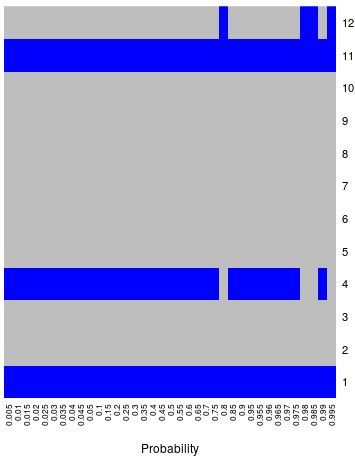
\includegraphics[width=0.4\linewidth]{Figuras/betas-mip/heatmap-exemplo-grupos}
%	\caption{}
%	\label{fig:heatmap-exemplo-grupos}
%\end{figure}
%
%
%\begin{eqnarray}
%\underset{\beta_{0\alpha},\beta_\alpha,z_{p \alpha}, \phi_{p \alpha}, \varepsilon_{t \alpha}^{+},\varepsilon_{t \alpha}^{-}}{\text{min}} & \sum_{\alpha \in A} \sum_{t\in T}\left(\alpha\varepsilon_{t \alpha}^{+}+(1-\alpha)\varepsilon_{t\alpha}^{-}\right) \label{eq:mipgr0} \\
%\mbox{s.t } & \varepsilon_{t \alpha}^{+}-\varepsilon_{t \alpha}^{-}=y_{t}-\beta_{0 \alpha}-\sum_{p=1}^{P}\beta_{p \alpha}x_{t,p},& \qquad\forall t \in T ,\forall \alpha \in A, \label{eq:mipgr1}\\
%& \varepsilon_{t \alpha}^{+},\varepsilon_{t \alpha}^{-}\geq0,&\qquad\forall t \in T ,\forall \alpha \in A, \label{eq:mipgr2}\\
%& - M z_{p \alpha} \leq \beta_{p \alpha} \leq M z_{p \alpha},&\qquad \forall \alpha \in A, \forall p\in\{1,\dots,P\}, \label{eq:mipgr3}\\
%& \sum_{p=1}^P z_{p \alpha} \leq K, & \qquad \forall \alpha \in A, \label{eq:mipgr4}\\
%& z_{p \alpha} \in \{0,1\},&\qquad \forall \alpha \in A, \forall p\in\{1,\dots,P\}, \label{eq:mipgr5}\\
%& \beta_{0\alpha} + \beta_{\alpha}^T x_{t} \leq \beta_{0\alpha'} + \beta_{\alpha'}^T x_{t}, & \qquad \forall t \in T, \forall (\alpha, \alpha') \in A \times A,  \alpha < \alpha',\nonumber\\ \label{eq:mipgr6} \\
%& z_{p\alpha} - z_{p\alpha+1} \leq m_{p\alpha}, & \qquad \forall \alpha \in A', \qquad \forall p \in P  \\
%& \sum_{\alpha \in A'} r_\alpha \leq |G| - 1 
%\label{eq:mipgr} \\
%\end{eqnarray}
%where $A' = A\setminus \{|A|\}$

\subsection{Best subset selection with LASSO}
\label{sec:best-subset-ell1}

Another way of doing regularization is including the $\ell_1$-norm of the coefficients on the objective function. The advantage of this method is that coefficients are shrunk towards zero by changing a continuous parameter $\lambda$, which penalizes the size of the $\ell_1$-norm.  
When the value of $\lambda$ gets bigger, fewer variables are selected to be used. 
This is the same strategy of the LASSO methodology, and its usage for the quantile regression is discussed in \cite{li2012l1}.
The proposed optimization problem to be solved is:
\begin{equation}
\underset{\beta_{0\alpha},\beta_\alpha}{\text{min}} \sum_{t \in T}\alpha|y_{t}-q_\alpha(x_t)|^{+}+ \sum_{t \in T}(1-\alpha)|y_{t}-q_\alpha(x_t)|^{-}+\lambda\|\beta_\alpha\|_{1},
\label{eq:l1-qar-optim}
\end{equation}
\[
q_\alpha(x_t)=\beta_{0}-\sum_{p=1}^{P}\beta_{p}x_{t,p}.
\]

For such estimation to be coherent, however, each covariate must have the same relative weight in comparison with one another. 
So, before solving the optimization problem, we perform a linear transformation such that all variables have mean $\mu = 0$ and variance $\sigma^2 = 1$. 
We apply the transformation $\tilde{x}_{t,p} = (x_{t,p} - \bar{x}_{t,p}) / \hat\sigma_{x_{t,p}}$, where $\bar{x}_{t,p}$ and $\hat{\sigma}_{x_{t,p}}$ are respectively the sample's unconditional mean and standard deviation. The $\tilde{y}_{t-p,i}$ series will be used to estimate the coefficients, as this series has the desired properties. 

After the process of normalization, we can rewrite problem \ref{eq:l1-qar-optim} as a LP problem, as shown below:
\begin{eqnarray}
\tilde \beta_\lambda^{*LASSO} = \underset{\beta_{0},\beta,\varepsilon_{t \alpha}^{+},\varepsilon_{t \alpha}^{-}}{\text{arg min}} & \sum_{\alpha \in A} \sum_{t \in T}\left(\alpha\varepsilon_{t \alpha}^{+}+(1-\alpha)\varepsilon_{t \alpha}^{-}\right)+\lambda\sum_{p=1}^{P}\mbox{\ensuremath{\xi}}_{p \alpha} \label{eq:obj-lasso} \\
\mbox{s.t. } & \varepsilon_{t \alpha}^{+}-\varepsilon_{t \alpha}^{-}= y_{t}-\beta_{0 \alpha}-\sum_{p=1}^{P}\beta_{p \alpha}\tilde x_{t,p},&\forall t\in T, \forall \alpha \in A, \\
& \varepsilon_{t \alpha}^{+},\varepsilon_{t \alpha}^{-}\geq0,&\forall t \in T, \forall \alpha \in A,\\
& \xi_{p\alpha}\geq\beta_{p \alpha},&\forall p\in P, \forall \alpha \in A,  \label{l1-qar-3}
\\
& \xi_{p\alpha}\geq-\beta_{p \alpha},&\forall p\in P, \forall \alpha \in A.  \label{l1-qar-4}
\end{eqnarray}
This model is built upon the standard linear programming model for the quantile regression (\ref{eq:linear-opt-1})-(\ref{eq:linear-opt-ult}). 
On the above formulation, the $\ell_1$ norm of equation (\ref{eq:l1-qar-optim}) is substituted by the sum of $\xi_p$, which represents the absolute value of $\beta_{p\alpha}$. The link between variables $\xi_p$ and $\beta_{p\alpha}$ is made by constraints (\ref{l1-qar-3}) and (\ref{l1-qar-4}). Note that the linear coefficient $\beta_{0\alpha}$ is not included in the penalization, as the sum of penalties on the objective function \ref{eq:obj-lasso}.

% % % % % % % % Esse trecho deve ser usado quando os coeficientes do lasso forem utilizados, e não apenas o lasso sendo um seletor de variáveis % % % % % % % % %
%Each component of the output $\tilde \beta_\lambda^{*LASSO}$ must be corrected by multiplying each coefficient for its standard deviation: $\beta_{p\alpha,\lambda}^{*LASSO} = \tilde \beta_{p\alpha,\lambda}^{*LASSO} \hat\sigma_{x_{t,p}}$.
%\begin{eqnarray}
%\tilde \beta_\lambda^{*LASSO} = \underset{\beta_{0},\beta,\varepsilon_{t \alpha}^{+},\varepsilon_{t \alpha}^{-}}{\text{arg min}} & \sum_{\alpha \in A} \sum_{t \in T}\left(\alpha\varepsilon_{t \alpha}^{+}+(1-\alpha)\varepsilon_{t \alpha}^{-}\right)+\lambda\sum_{p=1}^{P}\mbox{\ensuremath{\xi}}_{p \alpha} \label{eq:obj-lasso} \\
%\mbox{s.t. } & \varepsilon_{t \alpha}^{+}-\varepsilon_{t \alpha}^{-}= y_{t}-\beta_{0 \alpha}-\sum_{p=1}^{P}\beta_{p \alpha}\tilde x_{t,p},&\forall t\in T, \forall \alpha \in A, \\
%& \varepsilon_{t \alpha}^{+},\varepsilon_{t \alpha}^{-}\geq0,&\forall t \in T, \forall \alpha \in A,\\
%& \xi_{p\alpha}\geq\beta_{p \alpha},&\forall p\in P, \forall \alpha \in A,  \label{l1-qar-3}
%\\
%& \xi_{p\alpha}\geq-\beta_{p \alpha},&\forall p\in P, \forall \alpha \in A.  \label{l1-qar-4}
%\end{eqnarray}



For low values of $\lambda$, the penalty over the size of coefficients is small. Because of that, the output of problem (\ref{eq:obj-lasso})-(\ref{l1-qar-4}) is a model where most coefficients have nonzero value. On the other hand, when the penalty on $\| \beta_\alpha \|_1$ is big, many covariates will have zero valued coefficients. When $\lambda$ approaches infinity, one has a constant model. 
For instance, the penalty isn't applied to the linear coefficient $\beta_{0\alpha}$. 

Even though we have coefficients that are estimated by this method, we don't use them directly. In fact, the LASSO coefficients are biased, so it is employed only as a variable selector. As so, the nonzero coefficient covariates will be the input of a unrestricted quantile regression problem, as in the linear programming problem (\ref{eq:linear-opt-1})-(\ref{eq:linear-opt-ult}). 
The set of selected indexes are given by
\begin{equation*}
L_\lambda = \{ p \in \{ 1,\dots,P \} | \; |\beta^{*LASSO}_{\lambda,p}| \neq 0  \}.
\end{equation*}
Hence, we have that, for each $p \in \{ 1,\dots,P \}$,
$$\beta^{*LASSO}_{\lambda,p} = 0 \Longrightarrow \beta^{*}_{\lambda,p} = 0.$$
The post-lasso coefficients $\beta_\lambda^*$ are the solution from the optimization problem given below:
\begin{equation}
\begin{aligned} (obj_{\lambda}^{*},\beta_{\lambda}^{*})\overset{(obj,var)}{\longleftarrow} \min_{\beta_0,\beta,\varepsilon_{t}^{+},\varepsilon_{t}^{-}} & \sum_{t \in T}\left(\alpha\varepsilon_{t}^{+}+(1-\alpha)\varepsilon_{t}^{-}\right) \\
\mbox{s.t. } & \varepsilon_{t}^{+}-\varepsilon_{t}^{-}=y_{t} - \beta_0 - \sum_{p\in L_\lambda} \beta_p x_{t,p},& \forall t\in T,\\
& \varepsilon_t^+,\varepsilon_t^- \geq 0, & \forall t \in T.
\end{aligned}
\label{eq:post-lasso}
\end{equation}
The variable $obj_{\lambda}^{*}$ receives the value of the objective function on its optimal solution.
In summary, the optimization in equation \ref{eq:l1-qar-optim} acts as a variable selection for the subsequent estimation, which is normally called the post-LASSO estimation \cite{belloni2009least}.


For the same quantile values, $\alpha$, we experimented on section \ref{sec:best-subset-mip} ($\alpha \in \{0.05, 0.1, 0.5, 0.9, 0.95\}$), we estimate the post-LASSO (from now on, we call it just LASSO, for simplicity). Figure \ref{fig:lasso-results} shows the path of variables for each $\alpha$-quantile. On the x-axis, we have the penalty $\lambda$ in a log scale. On the y-axis we have the size of coefficients. One can see how increasing $\lambda$ leads to a shrinking on the size of coefficients, up to a point where all coefficients are equal to 0.
\begin{figure}
	\centering
	\begin{minipage}[t]{0.4\linewidth}
		\centering
		\begin{minipage}[t]{\linewidth}
			\centering     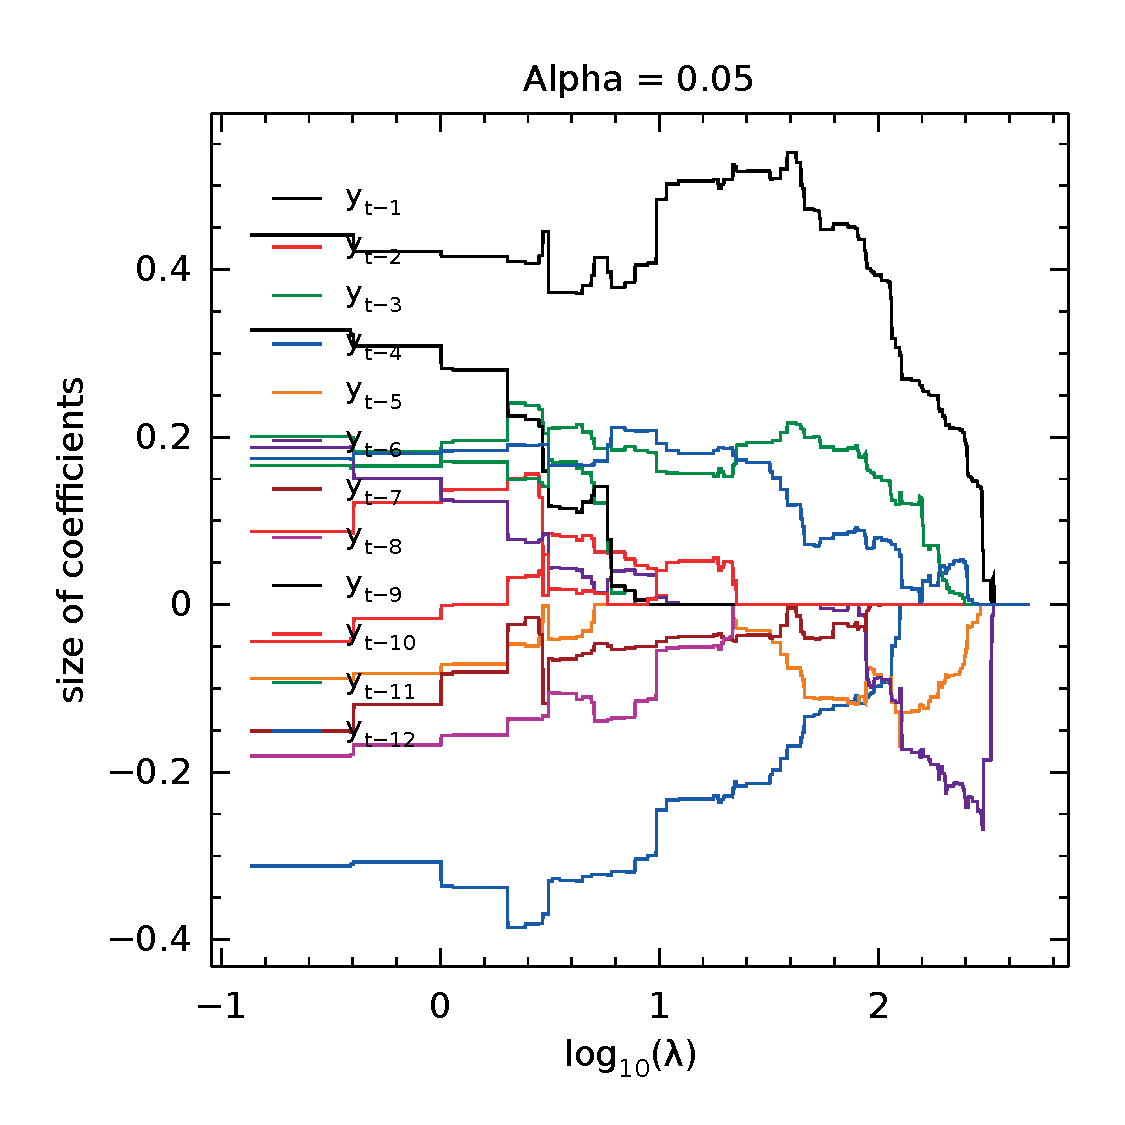
\includegraphics[width=\textwidth]{Figuras/selecao-lasso/par-sellasso-005.pdf}
		\end{minipage}
		\begin{minipage}[b]{\linewidth}
			\centering     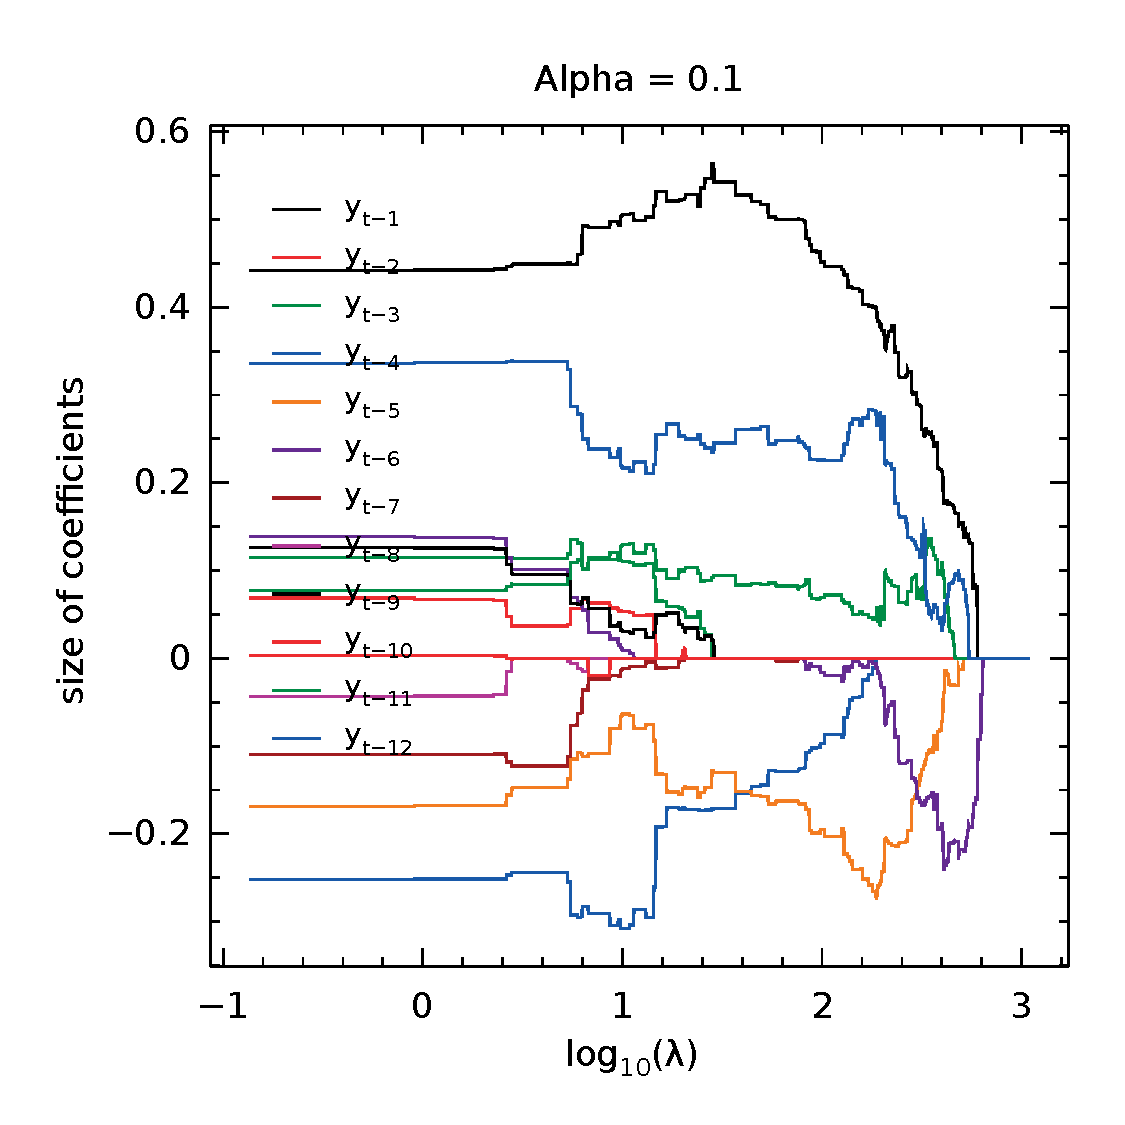
\includegraphics[width=\textwidth]{Figuras/selecao-lasso/par-sellasso-01.pdf}
		\end{minipage}
		\begin{minipage}[b]{\linewidth}
			\centering     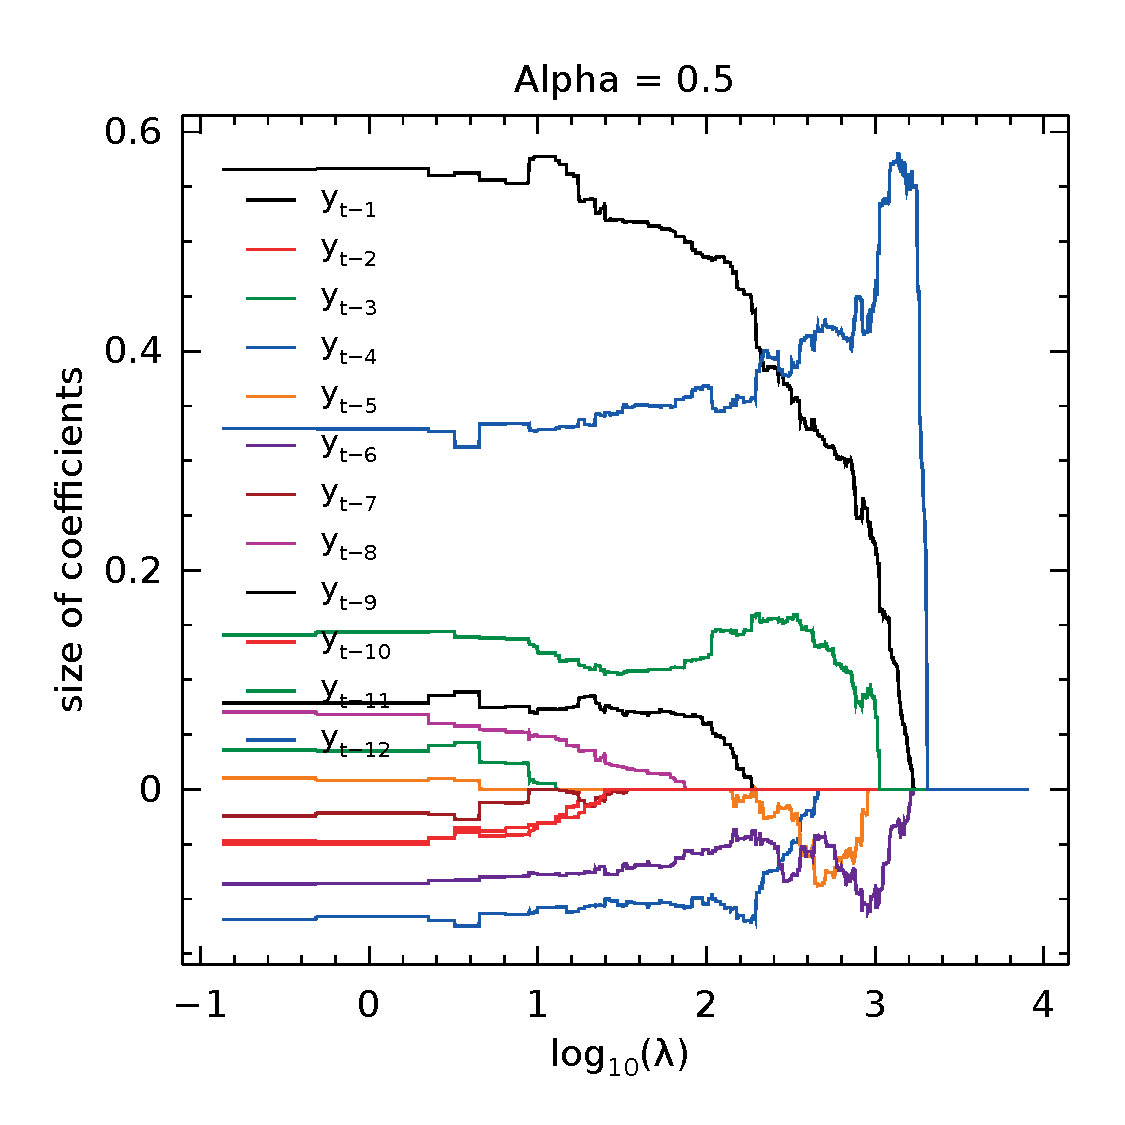
\includegraphics[width=\textwidth]{Figuras/selecao-lasso/par-sellasso-05.pdf}
		\end{minipage}
	\end{minipage}
	\begin{minipage}[t]{0.4\linewidth}
		\centering
		\begin{minipage}[b]{\linewidth}
			\centering     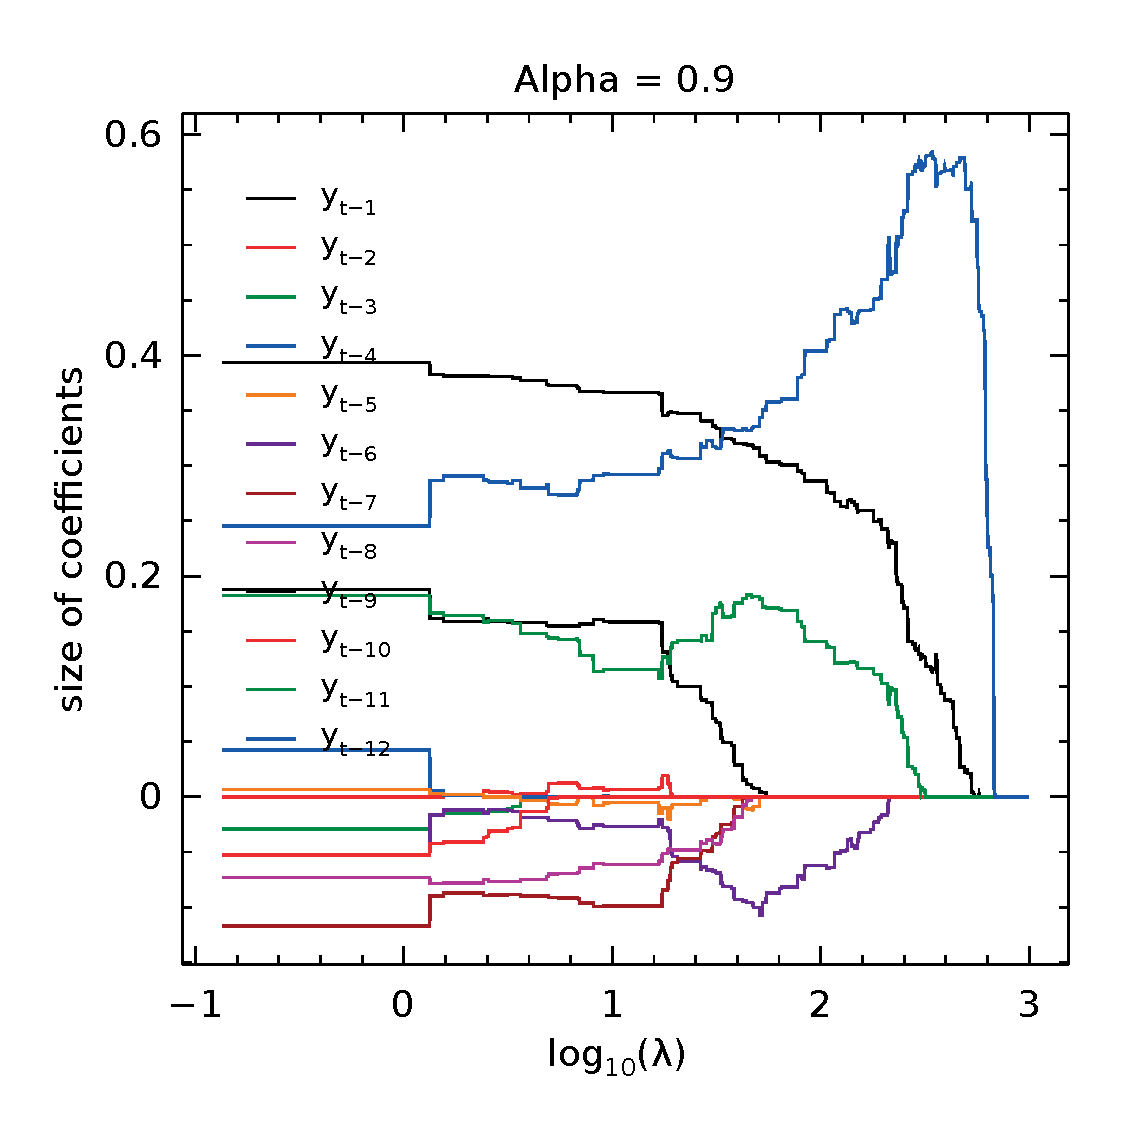
\includegraphics[width=\textwidth]{Figuras/selecao-lasso/par-sellasso-09.pdf}
		\end{minipage}
		\begin{minipage}[b]{\linewidth}
			\centering     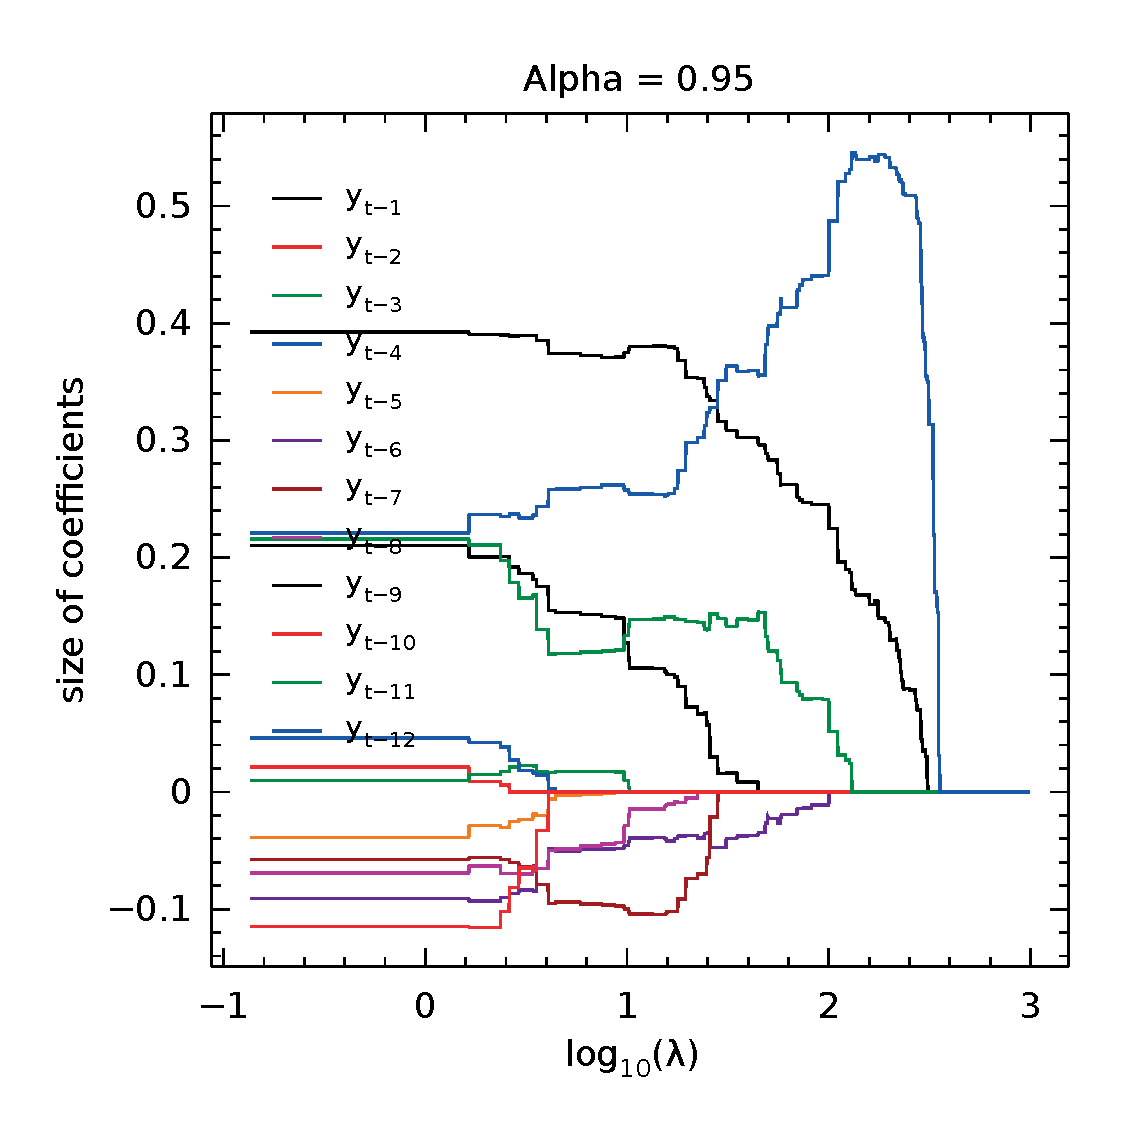
\includegraphics[width=\textwidth]{Figuras/selecao-lasso/par-sellasso-095.pdf}
		\end{minipage}
	\end{minipage}
	\caption{Coefficients path for a few different values of $\alpha$-quantiles. $\lambda$ is presented in a $\log_{10}$ scale, to make visualization easier.}
	\label{fig:lasso-results}
\end{figure}


\subsection{Model selection}

On sections \ref{sec:best-subset-mip} and \ref{sec:best-subset-ell1}, we presented two ways of doing regularization. Nonetheless, regularization can be done with different levels of parsimony. For example, one can select a different number $K$ of variables to be included in the best subset selection via MILP or choose different values of $\lambda$ for the $\ell_1$ penalty. 
%There is a tradeoff between variability and bias, when selecting the number of variables in a model. In order to  

% % % Métrica

Solving a LP problem is much faster than a similar-sized MILP problem. One of our goals is to test how much the LASSO approach gets close to the solution provided when solving the MILP problem. It would be interesting, then, if we could use a faster method that would provide a solution close to the best. To test how far are the solution given by both methods, we propose an experiment that is described as follows. Then, for each number $K$ of total nonzero coefficients, there will be a penalty $\lambda^*_K$ which minimizes the errors from the quantile regression's objective function (given on equation (\ref{eq:post-lasso})): 
%\todo{($K$ ranging from 0 until 12, where 0 means that only the intercept is included)}
\begin{equation}
\lambda^*_K = \argmin_\lambda \left\lbrace \left.  obj_{\lambda}^{*} \quad  \right| \, \| \beta^*_\lambda \|_0 = K \right\rbrace,
\end{equation}
where the quantity $\| \beta^*_\lambda \|_0$ is the $0$-norm, which gives the total of nonzero coefficients, for a given lambda of the LASSO estimations.

We, then, define the sets $L_K^{LASSO}$ and $L_K^{MILP}$, which contains all nonzero indexes, for a given $K$, when using methods LASSO and MILP for regularization, respectively.
Thus, we can compare the best LASSO fit where exactly $K$ variables are selected with the best fit given by the MILP problem, also with $K$ variables selected.

As the MILP solution is the exact solution for the problem, while the LASSO solution is an approximation, we use the former as a \textit{benchmarking} for the quality of the latter solution. To help us view the difference of results between both methods, we define a similarity metric $d$ between the subset of coefficients chosen by each one of them. It is desirable that the LASSO solution be as related with the MILP solution as possible.
The similarity is calculated as the solution of the following optimization problem
\begin{eqnarray}
d(\beta^*_{MILP(K)}, \beta^*_{\lambda^*_K}) = \min_{0\leq\delta_{ij}\leq1} & \sum\limits_{i,j = 1}^K  \delta_{ij} (1-|\rho_{ij}|) \label{eq:metricad0} \\
\text{s.t.} & \sum\limits_{j =1}^K\delta_{ij}=1, &  i=1,\dots,K,\\
& \sum\limits_{i =1}^K\delta_{ij}=1, & j=1,\dots,K,
\end{eqnarray}
where $\rho_{ij}$ is the correlation between the $i$-th and $j$-th independent variables in sets $L_k^{MILP}$ and $L_k^{LASSO}$, respectively. The optimal value for the decision variables of this problem provides us with an assignment between selected covariates from both methods, namely, MILP and LASSO, that minimizes the overall ``index of uncorrelation" between selected covariates. If $\delta^*_{ij} = 1$, the $i$-th selected variable in  $L_k^{MILP}$ is associated with the $j$-th variable  in $L_k^{LASSO}$. For instance, if $d(\beta^*_{MILP(K)}, \beta^*_{\lambda^*_K}) = 0$, it means that there are $K$ perfectly correlated pair of variables, despite not being the same.

% % % Trocar o sigma da função objetivo.




% % % recolocar no texto
As seen before, we have a best solution for each desired $K$. The question that arises now is how to select the ideal number of variables to use.
One way of achieving this is by using an information criteria to guide our decision. 
An information criteria summarizes two aspects. One of them refers to how well the model fits the in-sample observations. The other part penalizes the quantity of covariates used in the model. By penalizing how big our model is, we prevent overfitting from happening. So, in order for a covariate to be included in the model, it must supply enough goodness of fit.
In \cite{machado1993robust}, it is presented a variation of the Schwarz criteria for M-estimators that includes quantile regression. The Schwarz Information Criteria (SIC), adapted to the quantile autoregression case, is presented below:
\begin{align} 
\begin{split}
SIC(m) = n \log(\hat{\sigma}^*)+\frac{1}{2}K\log n,\label{eq:SIC}
\end{split}					
\end{align}
where $K$ is the model's dimension. This procedure leads to a consistent model selection if the model is well specified. 

Figure \ref{fig:comparison-lm-results} shows the results of these experiments for quantiles $\alpha \in \{0.05, 0.1, 0.5, 0.9, 0.95\}$. The results point us that for small values of $K$ the distance between coefficients is bigger and where we observe the biggest differences between the SIC values. In this experiment, the minimum SIC value for the MILP problem is usually found between 4 and 6 variables in the model.

\begin{figure}
	\centering
	\begin{minipage}[t]{0.4\linewidth}
		\centering
		\begin{minipage}[t]{\linewidth}
			\centering     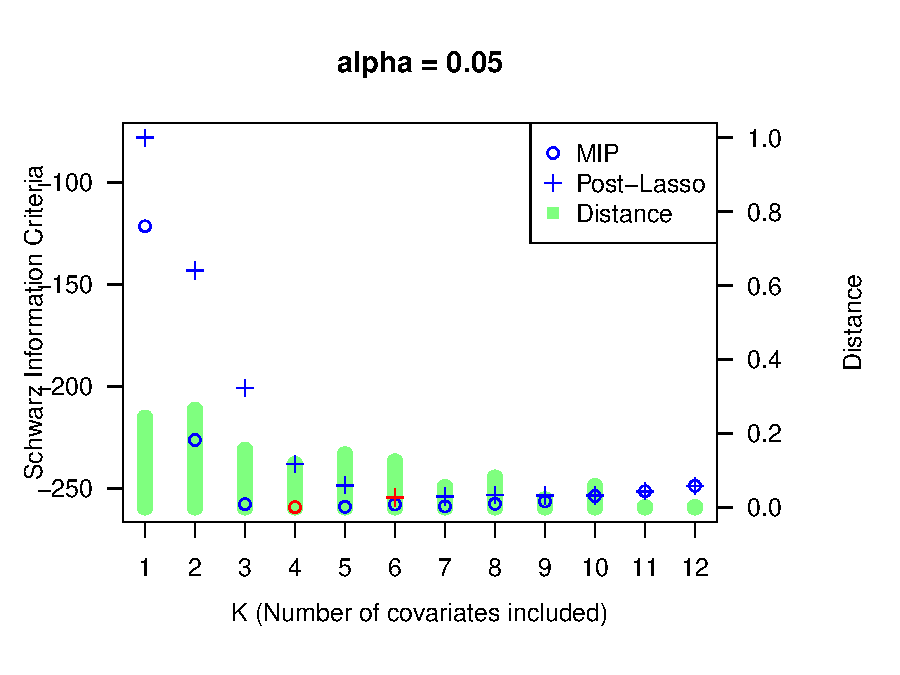
\includegraphics[width=\textwidth]{Figuras/SIC005.pdf}
		\end{minipage}
		\begin{minipage}[b]{\linewidth}
			\centering     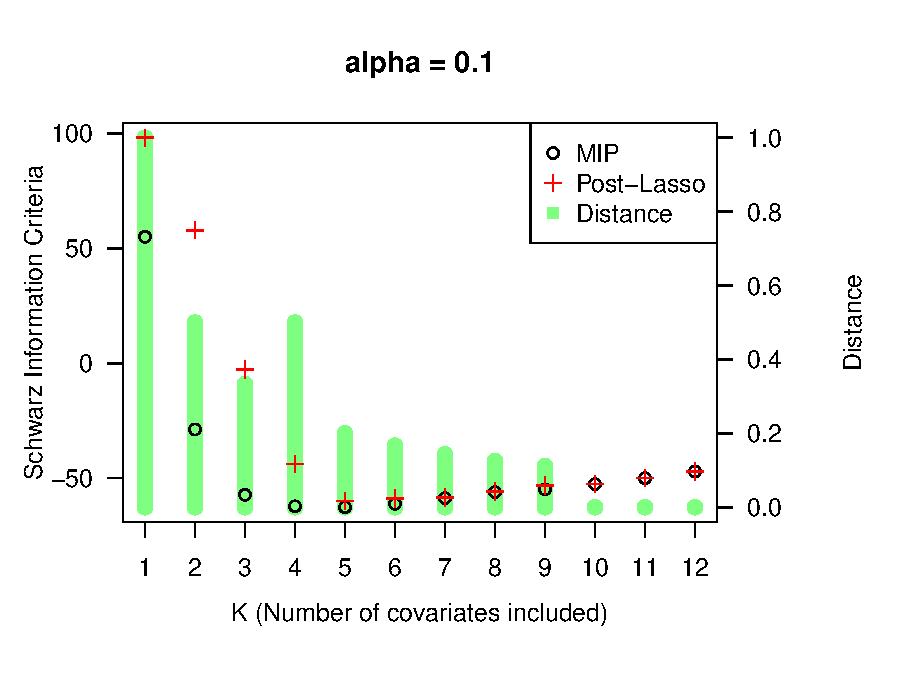
\includegraphics[width=\textwidth]{Figuras/SIC01.pdf}
		\end{minipage}
		\begin{minipage}[b]{\linewidth}
			\centering     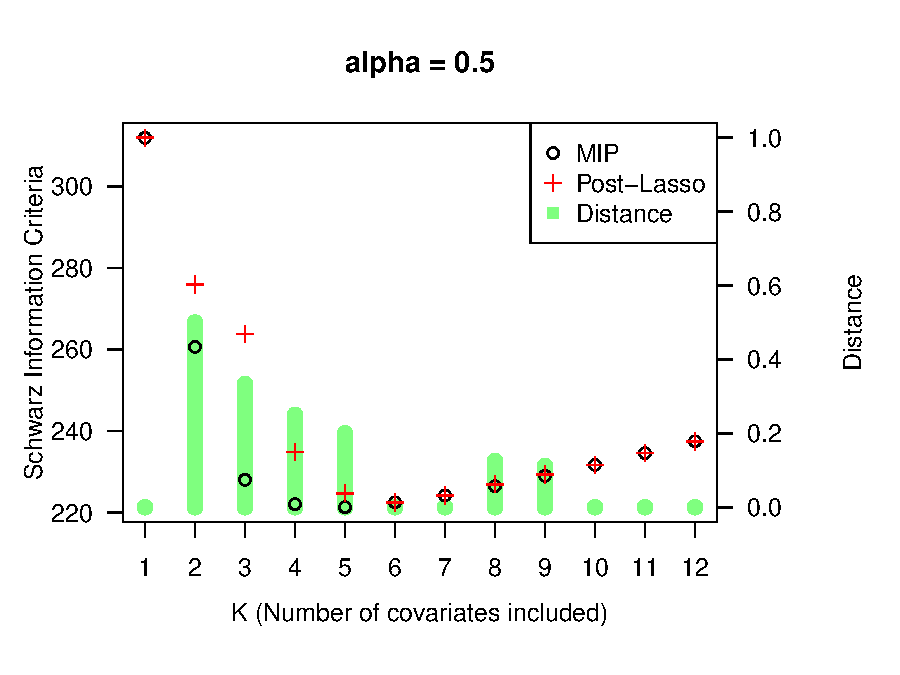
\includegraphics[width=\textwidth]{Figuras/SIC05.pdf}
		\end{minipage}
	\end{minipage}
	\begin{minipage}[t]{0.4\linewidth}
		\centering
		\begin{minipage}[b]{\linewidth}
			\centering     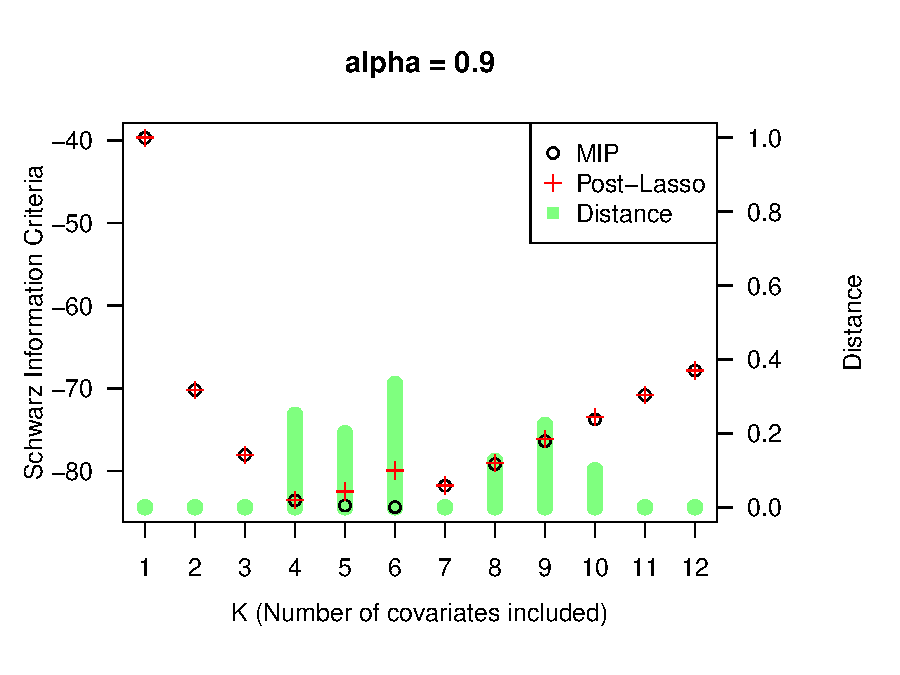
\includegraphics[width=\textwidth]{Figuras/SIC09.pdf}
		\end{minipage}
		\begin{minipage}[b]{\linewidth}
			\centering     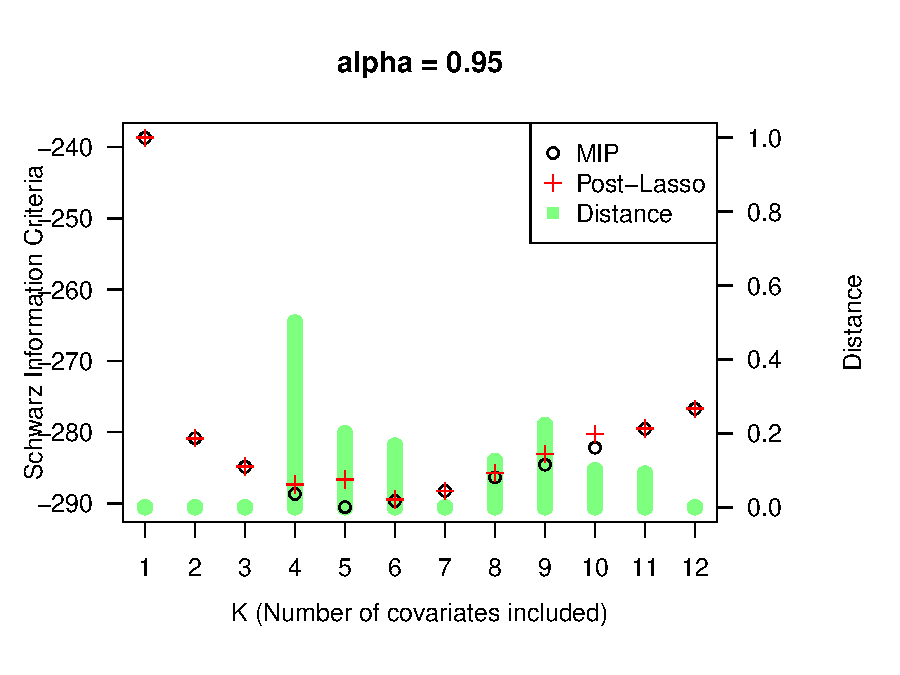
\includegraphics[width=\textwidth]{Figuras/SIC095.pdf}
			\label{fig:npqar-cross}
		\end{minipage}
	\end{minipage}
	\caption{ {Comparison of SIC values when using methods LASSO and MILP as a variable selector}. The Information Criteria is displayed on the y-axis, while the number of variables $K$ included is shown on the x-axis. Both solutions of the MILP and the best LASSO for a given $K$ are  The bars represent the distance $d$ as defined on problem (\ref{eq:metricad0})-(\ref{eq:metricad4}). When $d=0$, it means that the same variables are selected from both methods for a given $K$. Thus, in these cases we have the same SIC for both of them.}
	\label{fig:comparison-lm-results}
\end{figure}

